\documentclass[aspectratio=169,10pt]{beamer}
% Seven-slide, fully editable Beamer version of the accepted presentation.
% Numeric charts are PGFPlots, not screenshots. See data/*-exact.csv for fractions.
\usepackage[T1]{fontenc}
\usepackage{lmodern}
\usepackage{amsmath,booktabs,graphicx}
\usepackage{pgfplots}
\pgfplotsset{compat=1.18}
\usepackage{pgfpages}
\setbeameroption{hide notes} % Change to show notes on second screen for a speaker copy.
\definecolor{paper}{HTML}{F5F2E9}
\definecolor{ink}{HTML}{183F40}
\definecolor{muted}{HTML}{536563}
\definecolor{orange}{HTML}{AC4B34}
\definecolor{leaf}{HTML}{44745B}
\definecolor{gridline}{HTML}{DADFD4}
\definecolor{target}{HTML}{A8B59D}
\setbeamercolor{background canvas}{bg=paper}
\setbeamercolor{normal text}{fg=ink,bg=paper}
\setbeamercolor{frametitle}{fg=ink}
\setbeamercolor{structure}{fg=ink}
\setbeamercolor{footline}{fg=muted}
\setbeamercolor{itemize item}{fg=orange}
\setbeamerfont{frametitle}{size=\Large,series=\bfseries}
\setbeamertemplate{navigation symbols}{}
\setbeamertemplate{itemize item}{\small\raisebox{0.2ex}{\(\bullet\)}}
\setbeamersize{text margin left=7mm,text margin right=7mm}
\setbeamertemplate{frametitle}{\vspace{3mm}\insertframetitle\par\vspace{1mm}}
\setbeamertemplate{footline}{\hfill\usebeamerfont{footline}\tiny\insertframenumber\,/\,\inserttotalframenumber\hspace{5mm}\vspace{2mm}}
\newcommand{\smallsource}[1]{\par\vfill{\fontsize{6.4}{7.7}\selectfont\color{muted}#1\par}}
\newcommand{\claim}[1]{{\large\bfseries #1\par}}
\pgfplotsset{evidence/.style={
 width=9.8cm,height=5.15cm,
 axis line style={draw=gridline},tick style={draw=none},
 tick label style={font=\scriptsize,text=muted},
 label style={font=\scriptsize,text=ink},
 ymajorgrids=true,grid style={draw=gridline},
 axis background/.style={fill=paper},
 enlarge x limits=0.06,
 xlabel={Paired example (seed 907001--907012)},
 ylabel={Customer benefit difference},
 xtick={1,...,12},xticklabel style={font=\tiny},
 scaled ticks=false,/pgf/number format/fixed,
 ybar,bar width=3.6mm}}
% Keep this key outside frame bodies: Beamer captures frame contents in macros.
\pgfplotsset{legend image code/.code={\draw[#1] (0cm,-0.05cm) rectangle (0.20cm,0.10cm);}}
\hypersetup{pdftitle={When a local pricing guard is not a welfare promise},pdfauthor={Mohammadpayam Taebi and Arad Maleki},pdfsubject={AI Collusion Research Sprint; bounded pricing and welfare study}}
\begin{document}

% Slide 1 ------------------------------------------------------------------
\begin{frame}[plain]
\vspace{8mm}
{\fontsize{25}{29}\selectfont\bfseries When a local pricing guard\\is not a welfare promise\par}
\vspace{6mm}
{\large\color{muted}A model-specific study of customer protection\\and learned pricing behavior\par}
\vspace{11mm}
{\large\bfseries Mohammadpayam Taebi \quad Arad Maleki\par}
\vspace{1.5mm}
{\normalsize The Chinese University of Hong Kong (CUHK)\par}
\vspace{1.5mm}{\normalsize Team Boozines\par}
\note{Source: final report, title, abstract and Sections 1--8. Both authors are affiliated with CUHK; team name Boozines and coauthor Arad Maleki were supplied by the user. This is a bounded case study using established methods. It establishes neither stable collusion nor convergence nor a universal defense. Substantial AI development and drafting assistance is disclosed in the report; the current experiments use local tabular learners.}
\end{frame}

% Slide 2 ------------------------------------------------------------------
\begin{frame}[t]{The pricing game}
\begin{columns}[T,onlytextwidth]
\begin{column}{0.37\textwidth}
\vspace{1mm}
Two shops seek their own profit. Customers choose a shop or buy nothing.
\vspace{4mm}

The guard limits a proposed price using immediate profit against the rival's last price.
\vspace{4mm}

\claim{What customer benefit can it guarantee over many rounds?}
\end{column}
\begin{column}{0.60\textwidth}
\vspace{1mm}
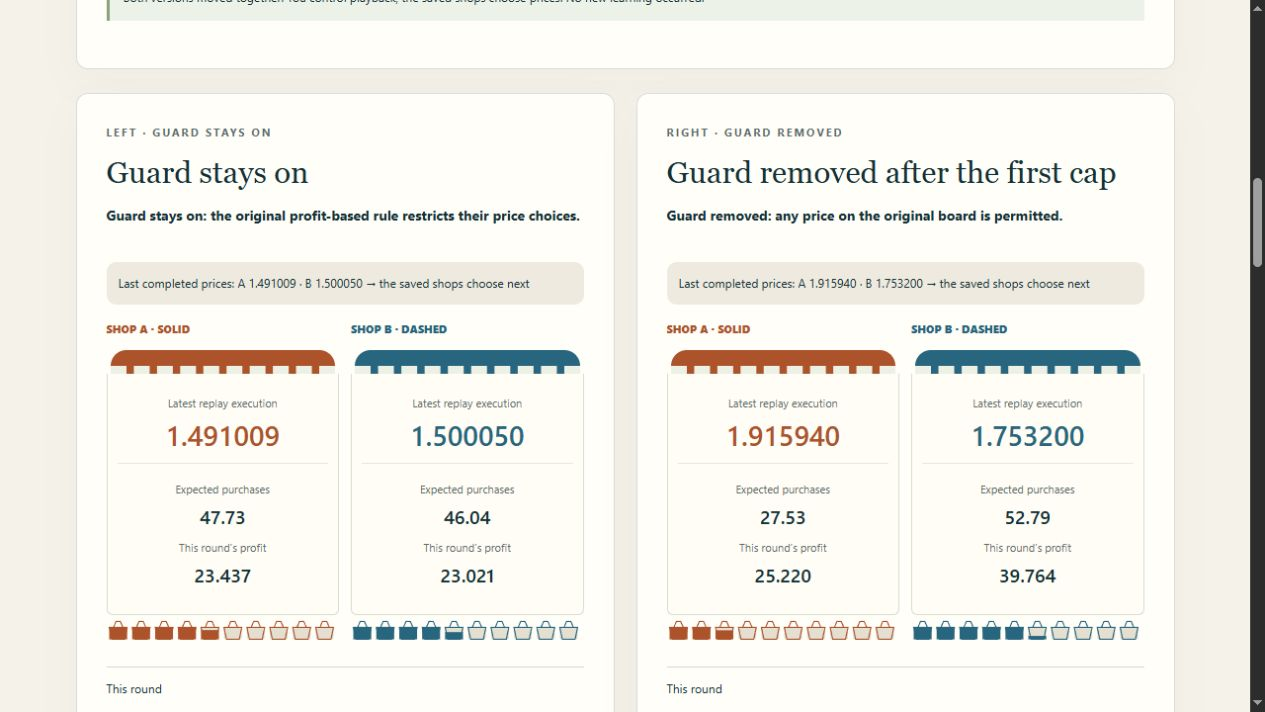
\includegraphics[width=\linewidth]{images/paired-replay.png}
\vspace{1.5mm}
{\scriptsize\color{muted}Actual replay: both worlds show prices, expected purchases and shop profits.}
\end{column}
\end{columns}
\smallsource{Screenshot: saved policies after learning; manual Play and saved-policy Watch are separate. Customer benefit means model consumer surplus.}
\note{Sources: research/PROBLEM\_DEFINITION.md; report Sections 1--2, 5, 7--8; research/GUARD\_REFERENCE\_REPLAY\_QA.md; original screenshot .local/guard-reference-v13-desktop.png. The screenshot is an illustration, not participant data. One click settles both saved worlds without exploration, updates, API calls or a fresh starting cap. The screenshot is copied byte-for-byte into images/paired-replay.png.}
\end{frame}

% Slide 3 ------------------------------------------------------------------
\begin{frame}[t]{Price precision changes the guarantee}
\begin{columns}[T,onlytextwidth]
\begin{column}{0.68\textwidth}
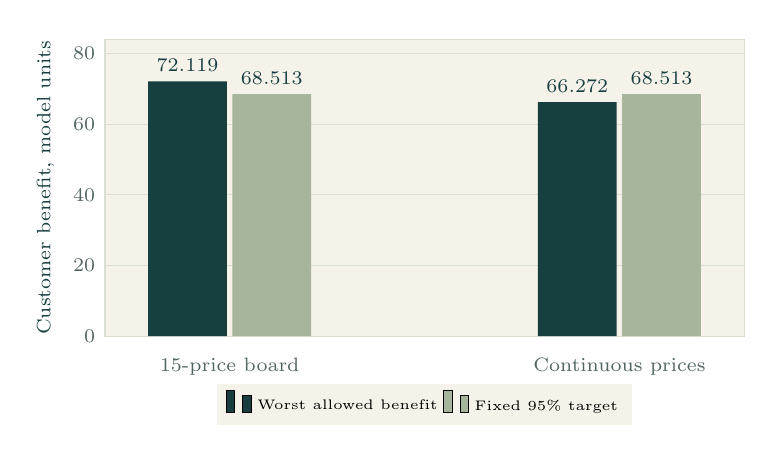
\begin{tikzpicture}
\begin{axis}[width=9.7cm,height=5.35cm,ybar,bar width=10mm,
 ymin=0,ymax=84,ytick={0,20,40,60,80},
 symbolic x coords={15-price board,Continuous prices},xtick=data,
 enlarge x limits=0.32,axis line style={draw=gridline},tick style={draw=none},
 tick label style={font=\scriptsize,text=muted},
 ylabel={Customer benefit, model units},ylabel style={font=\scriptsize,text=ink},
 ymajorgrids=true,grid style={draw=gridline},
 nodes near coords,nodes near coords style={font=\scriptsize,text=ink},
 /pgf/number format/fixed,/pgf/number format/precision=3,
 legend style={draw=none,fill=paper,font=\tiny,at={(0.5,-0.16)},anchor=north,legend columns=2},
 axis background/.style={fill=paper}]
\addplot[draw=none,fill=ink] coordinates {(15-price board,72.119) (Continuous prices,66.272)};
\addplot[draw=none,fill=target] coordinates {(15-price board,68.513) (Continuous prices,68.513)};
\legend{Worst allowed benefit,Fixed 95\% target}
\end{axis}
\end{tikzpicture}
\end{column}
\begin{column}{0.29\textwidth}
\vspace{4mm}
{\fontsize{27}{30}\selectfont\bfseries\color{orange}66.272\par}
\vspace{2mm}
\claim{falls below the 68.513 target}
\vspace{5mm}
The same initial cap. Separate finite and continuous calculations.
\end{column}
\end{columns}
\smallsource{Report \S3. Bounds shown rounded. These concern all permitted continuations, not observed learning.}
\note{Source: report Section 3 and continuous-refinement evidence. The economic calibration and physical starting cap are unchanged. The coarse 15-price finite guarantee is about 72.119, the continuous one-cap floor about 66.272, and the unchanged 95 percent target 68.513. Directed numerical bounds and exact saved finite-graph values have distinct scopes. This does not transfer the finite-grid certificate to continuous actions and makes no global controller-optimality claim. The plotted values preserve the rounded numbers in the original deck.}
\end{frame}

% Slide 4 ------------------------------------------------------------------
\begin{frame}[t]{Keeping the guard helps these learners}
\begin{columns}[T,onlytextwidth]
\begin{column}{0.70\textwidth}
\begin{tikzpicture}
\begin{axis}[evidence,ymin=-16,ymax=0,ytick={-16,-12,-8,-4,0}]
\addplot[draw=none,fill=orange] table[x=pair,y=difference]{data/reference.dat};
\end{axis}
\end{tikzpicture}
\end{column}
\begin{column}{0.27\textwidth}
\vspace{2mm}
{\fontsize{27}{30}\selectfont\bfseries\color{orange}$-12.733$\par}
\vspace{1mm}
Full grid after cap minus guard kept
\vspace{4mm}

\claim{All 12 favor keeping the guard}
\vspace{3mm}
{\small Same initial cap, clock, allocated memory and 2M-round budget.}
\end{column}
\end{columns}
\smallsource{One calibration and finite budget. More legal prices change learning difficulty. Mean and bars are descriptive; no confidence interval.}
\note{Sources: research/guard-reference-results/analysis.json, pairedRows and primarySummary; research/GUARD\_REFERENCE\_RESULTS.md; report Section 7. Every seed 907001--907012 is retained in source order. Chart bars round to six decimals; data/reference-exact.csv retains the exact rational differences. The mean is exactly -71666694001597459430390540863/5628433844731135543109222400, about -12.733. Guard mean 69.870422; full-grid mean 57.137449. Training and frozen execution constraints both change. Equal allocation and rounds do not imply equal competence. The full grid is the original bounded 62-price set. All 12 new trajectories and 24 checkpoints passed independent 24M-round replay. This is not evidence of convergence, stable collusion or a population effect. Three of twelve customer-benefit endpoints change between 1M and 2M rounds.}
\end{frame}

% Slide 5 ------------------------------------------------------------------
\begin{frame}[t]{Repeating the cap adds further benefit}
\begin{columns}[T,onlytextwidth]
\begin{column}{0.70\textwidth}
\begin{tikzpicture}
\begin{axis}[evidence,ymin=0,ymax=2.25,ytick={0,0.5,1,1.5,2}]
\addplot[draw=none,fill=leaf] table[x=pair,y=difference]{data/matched.dat};
\end{axis}
\end{tikzpicture}
\end{column}
\begin{column}{0.27\textwidth}
\vspace{2mm}
{\fontsize{27}{30}\selectfont\bfseries\color{leaf}$+0.956$\par}
\vspace{1mm}
Recurring cap minus startup guard
\vspace{4mm}

\claim{All 12 favor repeating the cap}
\vspace{3mm}
{\small Five clock labels and equal allocated memory in both arms.}
\end{column}
\end{columns}
\smallsource{Separate 24-run contrast. Every cycle-benefit endpoint changes between 1M and 2M rounds; no convergence claim.}
\note{Sources: research/matched-clock-results/analysis.json; research/MATCHED\_CLOCK\_RESULTS.md; report Sections 5--6. Exact mean 2420783571316325/2533274790395904, about +0.955595. All 12 seeds retained. Chart bars round to six decimals; data/matched-exact.csv retains the exact fractions. Initial phase 0 occurs once, then public phases 1--4 cycle. Recurring enforcement caps phase 4; startup guard keeps the guard. Both use 2M rounds, zero Q, full previous-price memory and paired streams. Independent replay covers 24 runs, 48 checkpoints and 48M rounds. This contrasts ongoing rule support during training and execution; it does not isolate policy formation or frequency alone. No new confidence interval.}
\end{frame}

% Slide 6 ------------------------------------------------------------------
\begin{frame}[t]{Methods and verification}
\vspace{1mm}
\claim{The shops use established tabular Q-learning}
\vspace{2mm}
\[
 Q(s,a)\leftarrow Q(s,a)+0.1\!\left[r+0.95\max_{a'\in\mathcal{A}(s')}Q(s',a')-Q(s,a)\right]
\]
\vspace{1mm}
Exact saved-weight graph arithmetic measures the frozen repeating patterns.
\vspace{5mm}
\begin{center}
\renewcommand{\arraystretch}{1.4}
\begin{tabular}{@{}lrrr@{}}
\toprule
\textbf{Study}&\textbf{Runs}&\textbf{Rounds replayed}&\textbf{Checkpoints}\\
\midrule
Recurring cap&24&48 million&48\\
Guard removal&12&24 million&24\\
\bottomrule
\end{tabular}
\end{center}
\smallsource{Separate implementations share V8 / Math.exp. The older 192-run study retains narrower replay coverage. These are verification counts, not extra samples.}
\note{Sources: report Sections 2, 5--7 and execution appendices; research/GUARD\_REFERENCE\_PROTOCOL.md; research/MATCHED\_CLOCK\_PROTOCOL.md; accepted independent-audit.json files. Training uses binary64 Q coefficients; saved-weight graph values use exact rational arithmetic. Firms select simultaneously from the last completed history; next-state bootstrap is captured before either update. New studies freeze sources and inventories before execution. Separate code replays all 72M distinct rounds across these two studies; repeated engineering verification adds no scientific sample. The V13 package's 91 checks are software/verification checks, not 91 market experiments. Shared V8, Math.exp and serialization libraries limit cross-runtime independence. The earlier 192-run study does not have this full-training-replay coverage.}
\end{frame}

% Slide 7 ------------------------------------------------------------------
\begin{frame}[t]{Contribution, limits and the game}
\begin{columns}[T,onlytextwidth]
\begin{column}{0.42\textwidth}
\claim{Contribution}
A controlled case linking a welfare guarantee to what pricing learners actually do.
\vspace{4mm}

\claim{Limits}
One model and budget. One full-grid shop earns below static Nash. Dynamic incentives and continued adaptation remain open.
\end{column}
\begin{column}{0.55\textwidth}
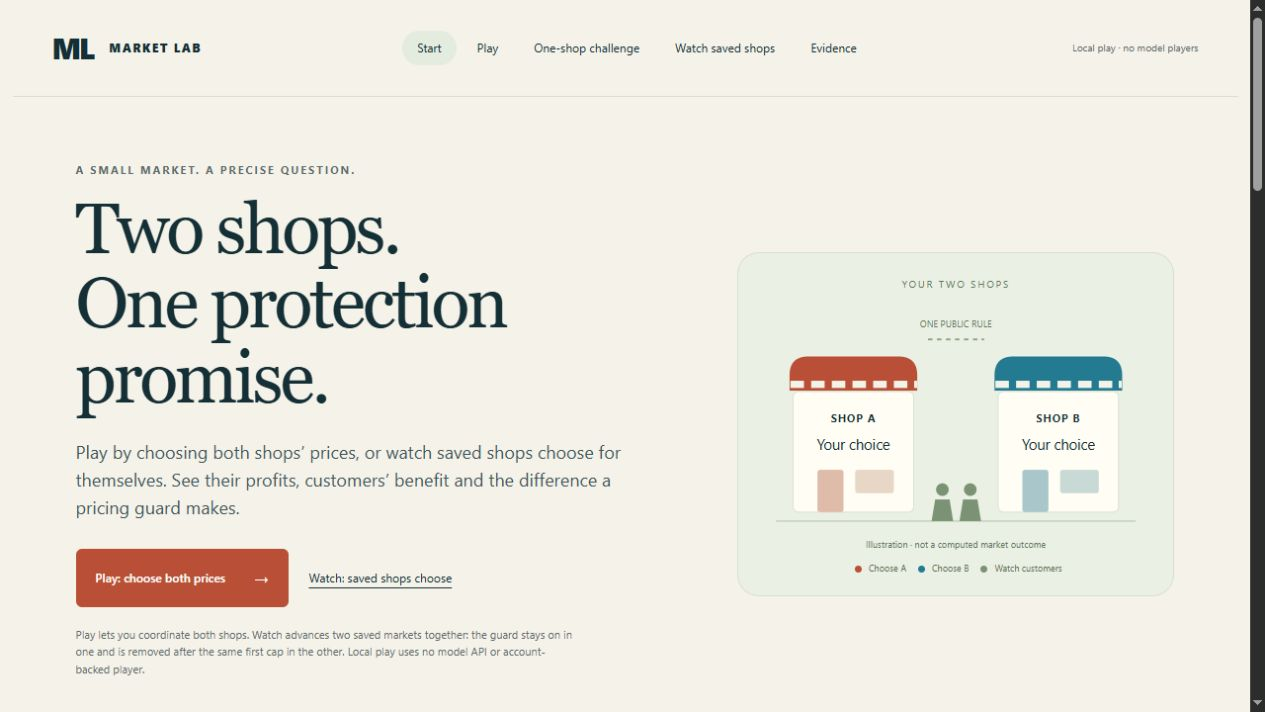
\includegraphics[width=\linewidth]{images/game-start.png}
\vspace{1.5mm}
\textbf{Play:} choose both prices.\\
\textbf{Watch:} saved shops choose.
\end{column}
\end{columns}
\smallsource{Play online: \url{https://aqapayam.github.io/local-pricing-guard/}. Code/setup: \url{https://github.com/aqaPayam/local-pricing-guard}. Full methods, prior work, limitations and substantial AI assistance are disclosed in the report.}
\note{Sources: report Sections 7--8 and ethical/AI-use appendix; research/GUARD\_REFERENCE\_RESULTS.md; research/CURRENT\_DEMO\_WALKTHROUGH.md; original .local/guard-reference-v13-start.png. The starter already supplies checkpoint branches, replacement, history windows and objective changes. Q-learning, shielding, renewal mixtures, safety budgets and frozen-partner dynamic programming are established methods, credited in the report. Our incremental contribution is the bounded pricing/control case and source-frozen comparisons. Static anchors are all pure Nash and exact joint-profit maxima on the original simultaneous table, not learned dynamic equilibria. 23/24 individual full-grid cycle profits exceed static Nash; seed 907009 Shop B earns 19.1434 against Nash 22.2927. The older 48-response audit does not cover these new reference cycles. Future work: broader economic calibrations and budgets; separate training/execution interventions; continued adaptation; dynamic incentive tests. No human usability study or experimental LLM player underlies these results. The local demo requires the separately supplied viewer and node research/demo-server.js. No external submission is implied.}
\end{frame}
\end{document}
